\documentclass{beamer}
\usepackage[utf8]{inputenc}
\usetheme{Warsaw}  %% Themenwahl
\usepackage{algpseudocode}
\usepackage{algorithm}
\usepackage{mathtools}

\title{Fehlerzustandsbaumanalyse}
\author{Öztürk Emrah, Schwartze Nicolai, Schneider Michael}
\date{\today}
\usepackage{amssymb}
\usepackage{float}

\begin{document}
\maketitle
%\frame{\tableofcontents[currentsection]}

\section{Allgemeine Informationen}
\frame{\tableofcontents[currentsection]}
\begin{frame}
	Definiertes Verfahren (EN 61025) zur Abschätzung der Ausfallswahrscheinlichkeit einer Anlage.\\~\\
	Breites Anwendungsgebiet in kritischen Branchen: Nuklearindustrie, Luft und Raumfahrt.\\~\\
	Basierend auf logischen Operationen und einfache Ausfallwahrscheinlichkeit.
\end{frame}


\begin{frame}
\begin{figure}
	\centering
	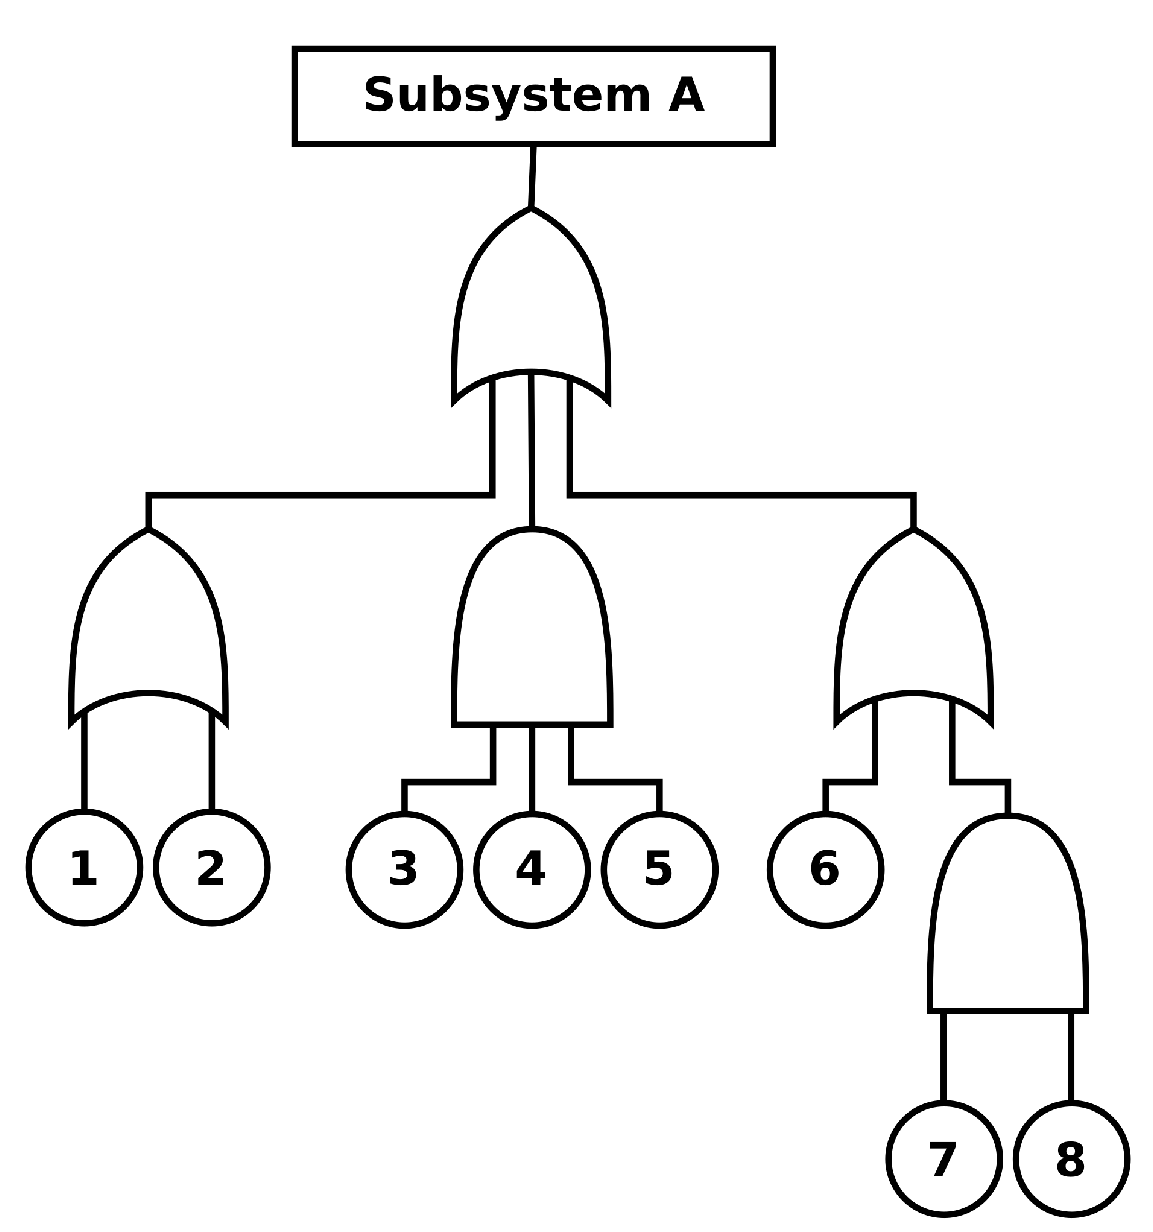
\includegraphics[width=0.6\linewidth]{fault_tree_example}
	\caption{Einfaches Fehlerzustandsbaumdiagramm Quelle: \href{https://en.wikipedia.org/wiki/Fault_tree_analysis}{https://en.wikipedia.org/wiki/Fault\textunderscore tree\textunderscore analysis}}
	\label{fig:faulttreeexample}
\end{figure}
\end{frame}

\begin{frame}
	
	
	
\end{frame}
	


\end{document}